\section{Preliminary Implementation} \label{sec:implementation}

We have implemented a prototype of \sysname on a testbed of clustered bare-metal
machines (Intel Xeon 2.40GHz 4-cores CPU, 67 GB RAM, 40Gbps Mellanox CX3 NIC,
CentOS 7). The prototype selects the most efficient data-plane mechanism based
on the location of two containers: if the two containers are intra-host,
shared-memory mechanism will be selected for data transfer, and if the two
containers are inter-host, RDMA will be selected.  We implemented the
shared-memory via multiplexing \texttt{IPC namespace}, and enabled containers to
use RDMA by using the \texttt{host mode}.  We evaluated our prototype and
compare it with state-of-the-art container overlay network - \texttt{Weave}. The
results are shown in Figure~\ref{fig:sys_eval_proto}. We see that the \sysname
prototype achieves higher throughput and lower latency. The CPU utilization per
bit/second is also significantly lower for \sysname compared to that of
\texttt{Weave}. 

\begin{figure}[ht]
\centering 
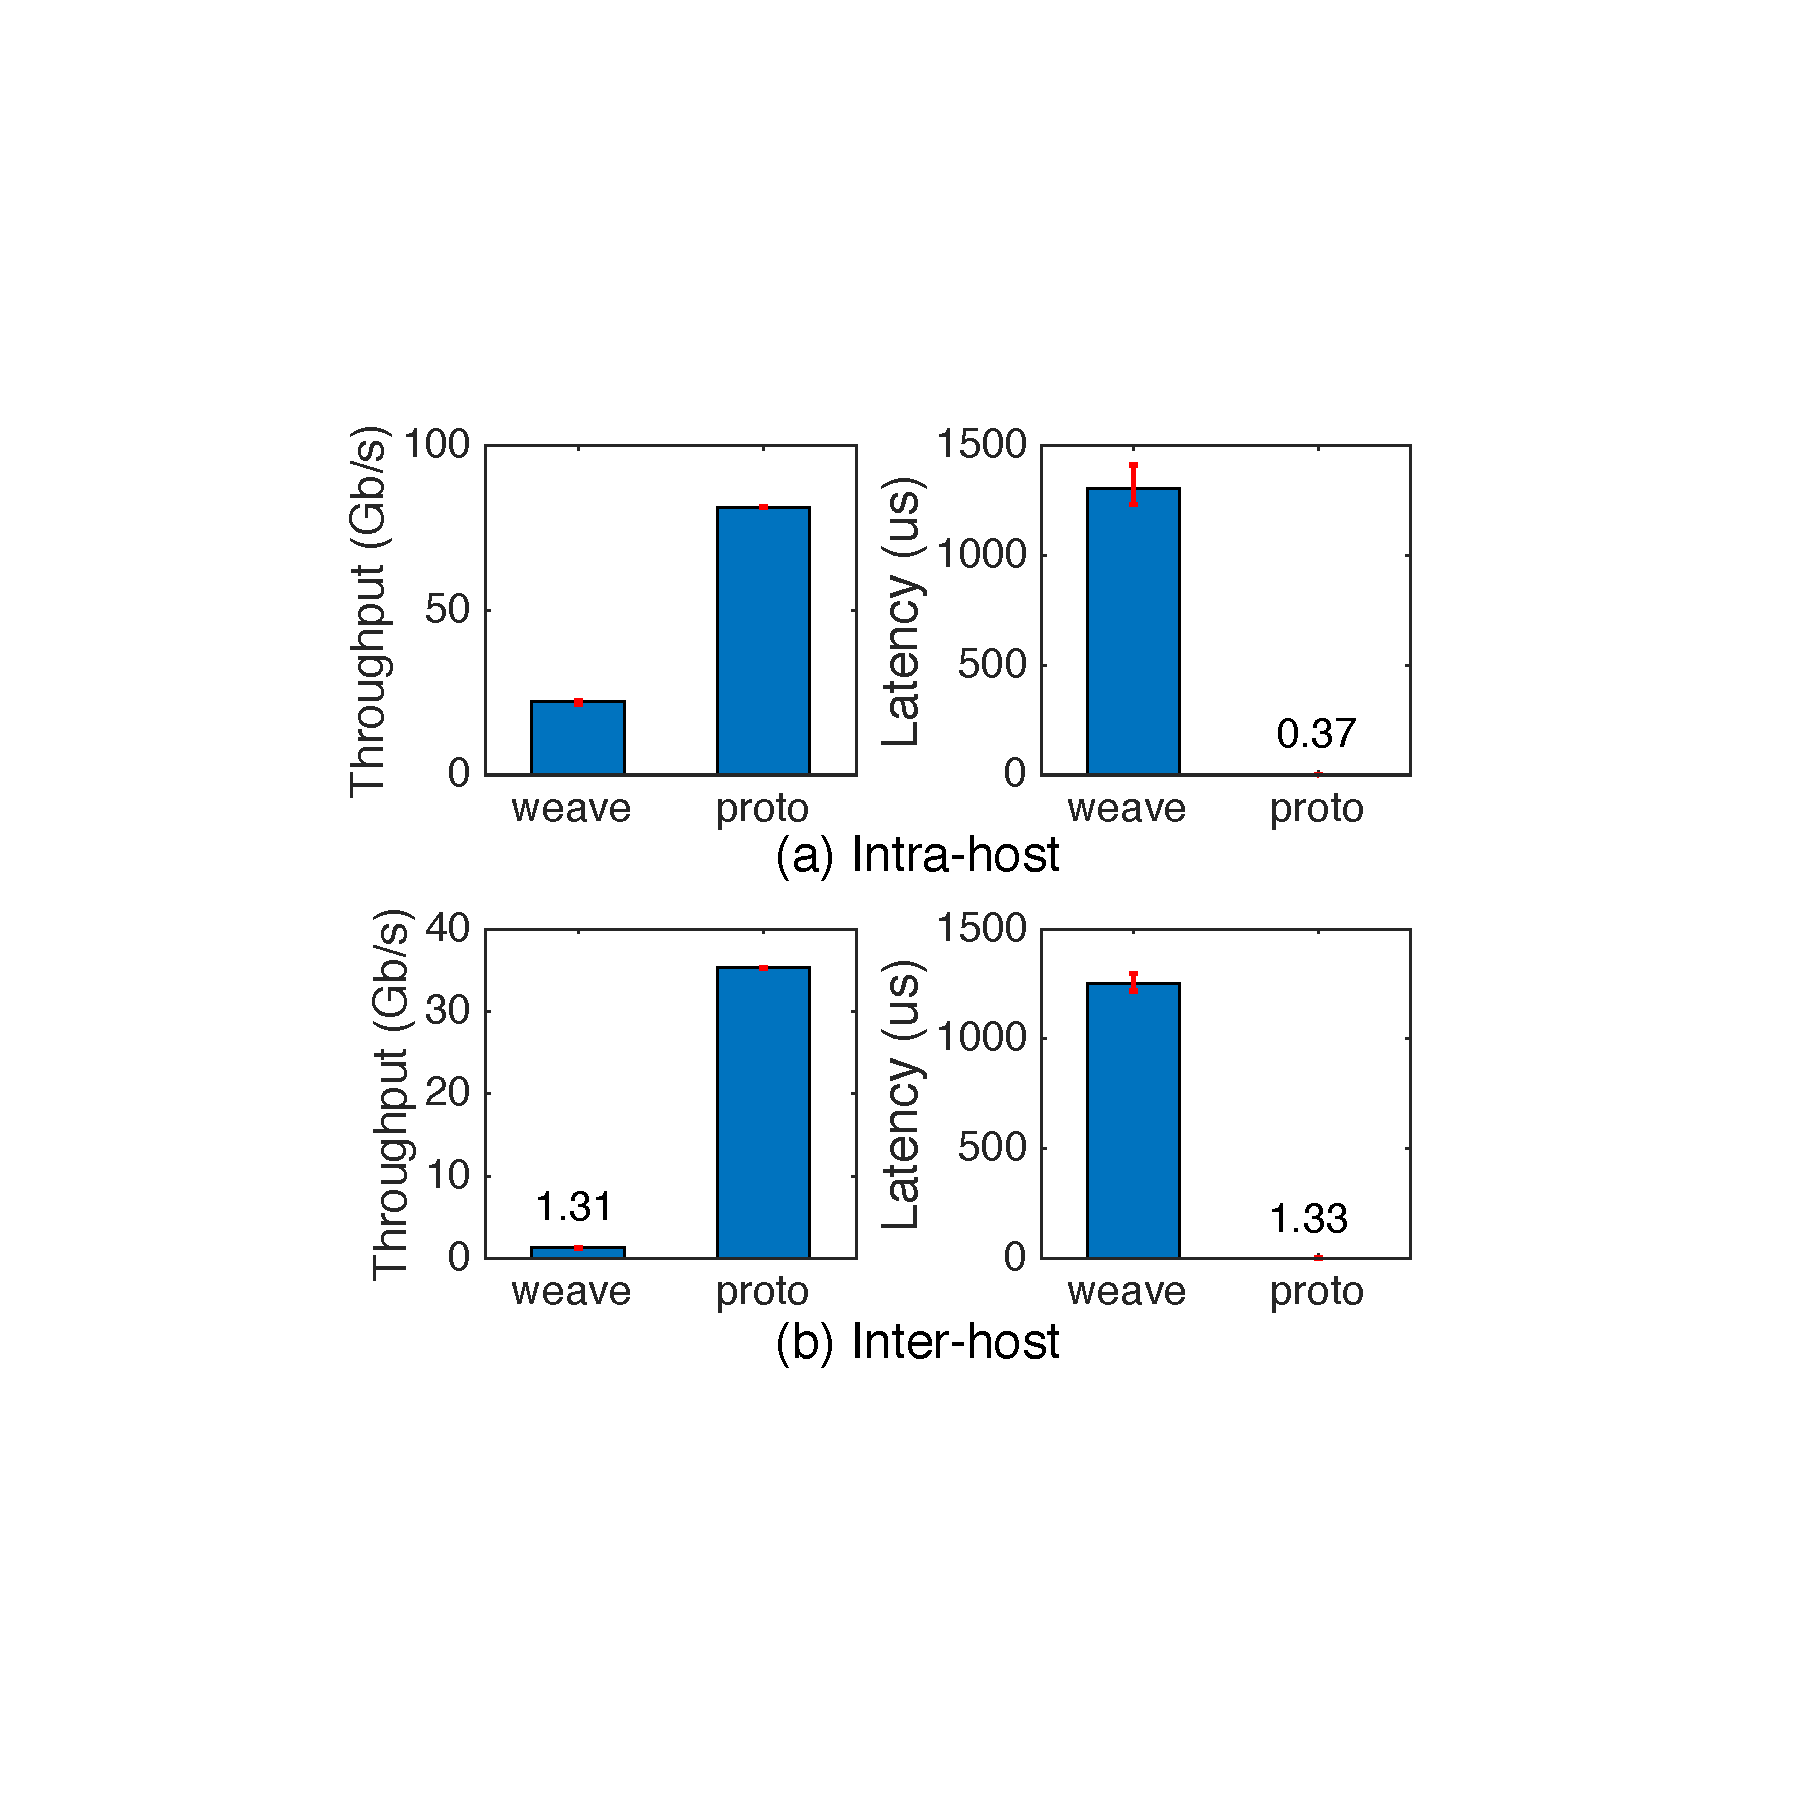
\includegraphics[width=0.45\textwidth]{figures/system/eval_proto.pdf}
\label{fig:sys_eval_proto}
\caption{Compare \sysname prototype with weave.} 
\end{figure}


